\documentclass[twoside,11pt,a4paper,openright]{article}
\usepackage[utf8]{inputenc}
\usepackage{amsmath}
\usepackage{listings}
\usepackage{pdfpages}
\usepackage{amsfonts}
\usepackage{caption}
%\usepackage{cite}
\usepackage{amssymb}
\usepackage[english]{babel}
\usepackage{fancyhdr}
\usepackage{graphicx}
%\usepackage{comment}
\usepackage{siunitx}
\usepackage{changepage}
\usepackage[rmargin=3cm,tmargin=3cm]{geometry}
%\usepackage[toc,page]{appendix}
%\usepackage{natbib}
%\usepackage{dsfont}
\usepackage{mathrsfs}
\usepackage{epstopdf}
\usepackage[labelfont=bf,width=0.92\textwidth]{caption}
% \usepackage{mathtools}
% \usepackage{breqn}
\usepackage{pbox}
\usepackage{upgreek}
\usepackage{epstopdf}
\usepackage{subcaption}
\usepackage{tikz}
\usetikzlibrary{arrows}
%\usetikzlibrary{angles}
\usepackage{etex}
%\usepackage{frcursive}
\usepackage{bm}
\setcounter{tocdepth}{2}
\newcommand{\skr}[1]{{\text{\small\slshape\cursive {#1}}}}
\newcommand{\fskr}[1]{\textbf{\pmb{\text{\small\slshape\cursive {#1}}}}}
\newcommand{\sech}{\text{sech}}
\newcommand{\diff}[3][]{\dfrac{\text{d}^{#1} #2}{\text{d} #3^{#1}}}
\newcommand{\pdiff}[3][]{\dfrac{\partial^{#1} #2}{\partial {#3}^{#1}}}
\newcommand{\lc}{\bigg\lbrace}
\newcommand{\rc}{\bigg\rbrace}
\newcommand{\ii}{\int_{-\infty}^{\infty}}
\newcommand{\ini}{\int_0^\infty}
\newcommand{\nk}[1][]{\vert u_{#1} \vert^2}
\newcommand{\pp}{\frac{\partial^2 \psi}{\partial t^2}}
\newcommand{\ppc}{\frac{\partial^2 \psi^*}{\partial t^2}}
\newcommand{\ppp}{\frac{\partial^3 \psi}{\partial t^3}}
\newcommand{\pppc}{\frac{\partial^3 \psi^*}{\partial t^3}}
\newcommand{\pppp}{\frac{\partial^4 \psi}{\partial t^4}}
\newcommand{\ppppc}{\frac{\partial^4 \psi^*}{\partial t^4}}
\newcommand{\imag}{\text{Im}}
\newcommand{\real}{\text{Re}}
\newcommand{\pt}{\partial_t}
\newcommand{\pz}{\partial_z}
\newcommand{\px}{\partial_x}
\newcommand{\pta}{\partial_{\tau}}
\newcommand{\pze}{\partial_{\zeta}}
\newcommand{\dtau}{\text{d}\tau}
\newcommand{\dx}{\text{d}x}
\newcommand{\dy}{\text{d}y}
\newcommand{\df}{\text{d}f}
\newcommand{\dt}{\text{d}t}
\newcommand{\dk}{\text{d}k}
\newcommand{\ddr}{\text{d}^Dr}
\newcommand{\divg}{\nabla \cdot}
\newcommand{\lap}{\nabla^2}
\newcommand{\zb}{\bar{z}}
\newcommand{\ub}{\bar{u}}
\newcommand{\tb}{\bar{t}}
\newcommand{\psit}[1]{\pt^{#1}\psi}
\newcommand{\la}{\mathcal{L}}
\newcommand{\sqp}{\sqrt{P_0}}
\newcommand{\nks}{|u|^{2\sigma}}
\newcommand{\nkst}{|u|^{2\sigma+2}}
\newcommand{\uc}{u^*}
\newcommand{\ue}{u_1}
\newcommand{\ut}{u_2}
\newcommand{\uez}{u_{1,z}}
\newcommand{\utz}{u_{2,z}}
\newcommand{\q}[1]{||#1||_{2}}
\newcommand{\sn}{\text{sn}}
\newcommand{\vb}{\bar{v}}
\setlength{\parindent}{0pt}
\setlength{\parskip}{1ex plus 0.5ex minus 0.2ex}
\pagestyle{fancy}
\fancyhead{}
\fancyhead[OR]{\fontsize{10}{12}\selectfont\nouppercase \thepage}
\fancyhead[ER]{\fontsize{10}{12}\selectfont\nouppercase \leftmark}
\fancyhead[OL]{\fontsize{10}{12}\selectfont\nouppercase \rightmark}
\fancyhead[EL]{\thepage}
\lstset{
  language=C,                % choose the language of the code
  numbers=none,                   % where to put the line-numbers
  stepnumber=1,                   % the step between two line-numbers.        
  numbersep=5pt,                  % how far the line-numbers are from the code
  backgroundcolor=\color{white},  % choose the background color. You must add \usepackage{color}
  showspaces=false,               % show spaces adding particular underscores
  showstringspaces=false,         % underline spaces within strings
  showtabs=false,                 % show tabs within strings adding particular underscores
  tabsize=2,                      % sets default tabsize to 2 spaces
  captionpos=b,                   % sets the caption-position to bottom
  breaklines=true,                % sets automatic line breaking
  breakatwhitespace=true,         % sets if automatic breaks should only happen at whitespace
  title=\lstname,                 % show the filename of files included with \lstinputlisting;
}

% \fontsize{10}{12}\selectfont\nouppercase\leftmark
\begin{document}
%%%%%%%%%%%%%%%%%%%%%%%%%%%%%%%%%%%%%%%%%
% University Assignment Title Page 
% LaTeX Template
% Version 1.0 (27/12/12)
%
% This template has been downloaded from:
% http://www.LaTeXTemplates.com
%
% Original author:
% WikiBooks (http://en.wikibooks.org/wiki/LaTeX/Title_Creation)
%
% License:
% CC BY-NC-SA 3.0 (http://creativecommons.org/licenses/by-nc-sa/3.0/)
% 
% Instructions for using this template:
% This title page is capable of being compiled as is. This is not useful for 
% including it in another document. To do this, you have two options: 
%
% 1) Copy/paste everything between \begin{document} and \end{document} 
% starting at \begin{titlepage} and paste this into another LaTeX file where you 
% want your title page.
% OR
% 2) Remove everything outside the \begin{titlepage} and \end{titlepage} and 
% move this file to the same directory as the LaTeX file you wish to add it to. 
% Then add \input{./title_page_1.tex} to your LaTeX file where you want your
% title page.
%
%%%%%%%%%%%%%%%%%%%%%%%%%%%%%%%%%%%%%%%%%

%----------------------------------------------------------------------------------------
%	PACKAGES AND OTHER DOCUMENT CONFIGURATIONS
%----------------------------------------------------------------------------------------

\begin{titlepage}

\newcommand{\HRule}{\rule{\linewidth}{0.5mm}} % Defines a new command for the horizontal lines, change thickness here

\center % Center everything on the page
 
%----------------------------------------------------------------------------------------
%	HEADING SECTIONS
%----------------------------------------------------------------------------------------

\textsc{\LARGE Technical University of Denmark}\\[1.5cm] % Name of your university/college
\textsc{\Large High-Performance Computing}\\[0.5cm] % Major heading such as course name
\textsc{\large Course 02614}\\[0.5cm] % Minor heading such as course title

%----------------------------------------------------------------------------------------
%	TITLE SECTION
%----------------------------------------------------------------------------------------

\HRule \\[0.4cm]
{ \huge \bfseries Assignment 2}\\[0.4cm] % Title of your document
\HRule \\[1.5cm]
 
%----------------------------------------------------------------------------------------
%	AUTHOR SECTION
%----------------------------------------------------------------------------------------

%\begin{minipage}{0.4\textwidth}
%\begin{flushleft} \large
%\emph{Author:}\\
%Mikkel \textsc{Jensen} % Your name
%\end{flushleft}
%\end{minipage}
~
%\begin{minipage}{0.4\textwidth}
%\begin{flushright} \large
%\emph{Supervisor:} \\
%Dr. James \textsc{Smith} % Supervisor's Name
%\end{flushright}
%\end{minipage}\\[4cm]

% If you don't want a supervisor, uncomment the two lines below and remove the section above
\Large \emph{Authors:}\\
Oskar \textsc{Hint}, s161559\\
Mikkel \textsc{Jensen}, s123184\\
Philip \textsc{Rasmussen}, s103124\\
[2cm] % Your name

%----------------------------------------------------------------------------------------
%	DATE SECTION
%----------------------------------------------------------------------------------------

{\large \today }\\[2cm] % Date, change the \today to a set date if you want to be precise

%----------------------------------------------------------------------------------------
%	LOGO SECTION
%----------------------------------------------------------------------------------------
\vspace{4cm}
\begin{center}
%\includegraphics[width=0.5\textwidth]{fig/dtufotoniklogo.png}
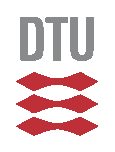
\includegraphics{fig/DTU_3_CMYK.eps}
\end{center}
 % Include a department/university logo - this will require the graphicx package
 
%----------------------------------------------------------------------------------------

\vfill % Fill the rest of the page with whitespace

\end{titlepage}
\newpage
\tableofcontents
\thispagestyle{empty}
\setcounter{page}{0}
\newpage
\section{Introduction}


\subsection{Specifications}

\section{Assignment}




\section{Conclusion}
We have implemented 6 functions all computing a matrix matrix product, and each having a different permutation of loop orders. Using different compiler optimizations, the best one was found to be mkn, topping at $\sim 1600$ MFlop/s, opposed to the DGEMM library function which tops at $\sim 22000$ MFlop/s. Cache hits and misses were analyzed to highlight the difference in performance between the permutations, and the analysis showed that the quickest functions has the highest hit-to-miss-ratio as expected. Finally, blocking was implemented as an attempt to better the performance degradation from the memory footprint exceeding the L3 cache size. The implementation was successful, but performance-wise, it only showed a minor improvement as opposed to the best non-blocked version. This is partly due to the Sun Studio compiler doing a great job at prefetching. However, we expect that the blocked version will be better than the non-blocked version for matrices larger than the one tested here.
\end{document}
